

\noindent{\bfseries\fontsize{16pt}{19.2pt}\selectfont ผลการทดสอบโมเดล}\par


\indent โมเดลสามารถจำแนกปลากัดทั้งสามกลุ่ม (ปลากัดพื้นบ้านภาคอีสานหางลาย, ปลากัดพื้นบ้านภาคใต้, ปลากัดพื้นบ้านมหาชัย) ได้อย่างถูกต้องบน
Validation set อย่างไรก็ตาม ขนาดข้อมูลยังค่อนข้างเล็กโดยเฉพาะคลาส ปลากัดพื้นบ้านมหาชัย ที่มีจำนวน
น้อย ซึ่งอาจทำให้โมเดลมี Bias และค่า Accuracy ที่ได้สูงอาจสะท้อน Overfitting ต่อโดเมนข้อมูล
ที่ใช้ ดังนั้นควรมีการทดสอบเพิ่มเติมกับชุดข้อมูลใหม่ที่ไม่ได้อยู่ในกระบวนการฝึก เพื่อประเมินความ
สามารถทั่วไป (generalization) ของโมเดล

\vspace{\baselineskip}

\begin{figure}[h]
	\centering
	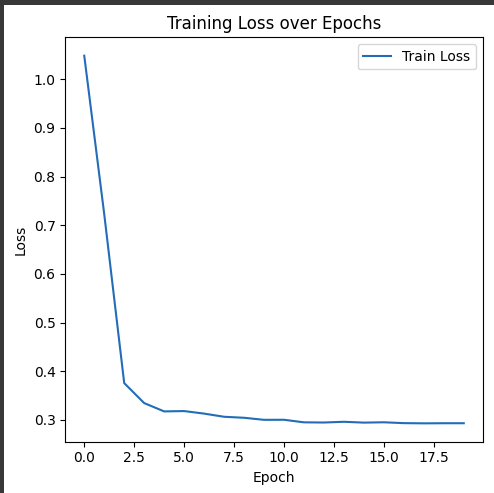
\includegraphics[width=0.47\linewidth]{GF2}
	\hfill
	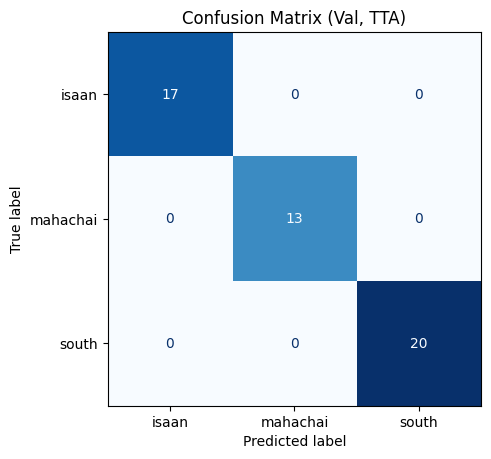
\includegraphics[width=0.47\linewidth]{GF1}
	\caption{กราฟ Loss ของ Train และ Validation และ Confusion Matrix ของผลการทดสอบ}
\end{figure}

\par\endgroup
\clearpage

%================== จบ Appendix.tex ====================